\documentclass[conference]{IEEEtran}
%\IEEEoverridecommandlockouts
% The preceding line is only needed to identify funding in the first footnote. If that is unneeded, please comment it out.
\usepackage[spanish]{babel}
\usepackage{cite}
\usepackage{amsmath,amssymb,amsfonts}
\usepackage{algorithmic}
\usepackage{graphicx}
\usepackage{textcomp}
\usepackage{xcolor}

\def\BibTeX{{\rm B\kern-.05em{\sc i\kern-.025em b}\kern-.08em
    T\kern-.1667em\lower.7ex\hbox{E}\kern-.125emX}}
\begin{document}

\title{Presentación Proyecto Final\\
{\Large Laboratorio de Sistemas Embebidos}
\thanks{Identify applicable funding agency here. If none, delete this.}
}

\author{\IEEEauthorblockN{Tatiana Felizia}
\IEEEauthorblockA{\textit{Prácticas Profesionalizantes} \\
\textit{E.E.S.T. N°7 "T.R.Q."}\\
Quilmes, Buenos Aires, Argentina\\
tatianafelizia@gmail.com}
\and
\IEEEauthorblockN{Lara Diaz Steinbrecher}
\IEEEauthorblockA{\textit{Prácticas Profesionalizantes} \\
\textit{E.E.S.T. N°7 "T.R.Q."}\\
Quilmes, Buenos Aires, Argentina \\
laradiazsteinbrecher@gmail.com}
} 

\maketitle

\begin{abstract}
    Este informe conforma el proyecto integrador del curso de Sistemas Embebidos realizado en la Universidad Tecnológica Nacional. El proyecto consiste en una aplicación que trabaja con FreeRTOS, integrando los periféricos del microcontrolador LPC845.
\end{abstract}

\begin{IEEEkeywords}
    Tareas, Sistema Operativo en Tiempo Real, Microcontrolador, Colas
    
\end{IEEEkeywords}

\section{Introducción}
    En este informe dará una íntegra explicación de proyecto integrador del curso de Sistemas Embebidos. El mismo busca integrar los conocimientos adquiridos a lo largo de la cursada con una aplicación en FreeRTOS, utilizando los periféricos del microcontrolador LPC845.\par

\section{Resumen}

El programa, desarrollado en C, alterna constantemente entre las distintas tareas que lo conforman utilizando el sistema de FreeRTOS, en cada tarea utilzia distintos periféricos, todos pertenecientes a una placa de desarrollo realizada en el laboratorio de la facultad. El microcontrolador que utiliza es un LPC845. EL proyecto fue desarrollado utilizando MCUXpresso.\par

\section{Desarrollo del programa}
    \subsection{Definición de Colas en FreeRTOS}
        El sistema utiliza 4 colas de FreeRTOS:
          \begin{itemize}
            \item queue\_setpoint\par
            \item queue\_boo\_var\par
            \item queue\_adc\par
            \item queue\_light\_intensity\par
        \end{itemize}
    
    \subsection{Definición de Tareas en FreeRTOS}
        Para asegurar que todas las tareas sean ejecutadas en tiempo real, el programa cuenta con una serie de tareas declaradas que utilizará alternando entre ellas de forma regular.\par

        \begin{itemize}
            \item task\_init:
            Es la función que inicializa los periféricos que serán utilizados por el programa: el puerto de I2C, el de ADC, el PWM y el display de 7 segmentos.\par
            Se trata de la primera función a ejecutar por el sistema, es la que más prioridad tiene. Su función es dar inicio al sistema.\par
            
            \item task\_BH1750: Realiza la lectura del sensor lumínico BH1750, en función de su resultado obtiene el valor de var, que variará en función del brillo del ambiente. Esta función es la que le entrega valores a la cola queue\_light\_intensity.\par

            \item task\_setpoint: Lee los valores de los pines de los botones 1 y 2, y según cuál de los dos esté presioado, incrementa o decrementa la variable setpoint, misma que agregará a una cola queue\_setpoint.\par
            Esta función también se asegura de que, el valor de setpoint se mantenga entre los valores estipulados, 25 y 75.\par
            
            \item task\_btn: Esta función lee constantemente el valor del pin del botón de user, al detectar un pulso invierte la variable boo. Posteriormente, guardará esta variable en la cola queue\_boo\_var.\par
            
            \item task\_display\_write: La finalidad del proyecto es alternar entre el valor de luminocidad (var) y el del setpoint (setpoint) en el display 7 segmentos al presionar el botón de user. Esto lo registramos en la función anterior, y ese dato lo guardamos en la cola queue\_boo\_var. Aquí recogemos este valor, y según cuál sea su valor, será el parámetro que mostraremos en el display: Si boo = 1, mostramos el valor de var; si boo = 0, mostramos el valor de setpoint.\par
            En cada uno de estos casos, la tarea recogerá los valores de las colas queue\_setpoint o el del queue\_light\_intensity\par
            Para mostrar cada parámetro en el display, la tarea primero apaga el display 7 segmentos, para luego encender el valor de las decenas, lo apaga, y enciende el de las unidades. Este proceso lo repite entre pequeños delays. A simple vista, no se alcanzan a observar las pausas.\par           
            \item task\_adc:
            Periódicamente, realiza conversiones del canal 0 del ADC.\par
            
            \item task\_blueled: Recoge los valores de la cola queue\_adc, donde residen los resultados de las conversiones del ADC. En función de este valor (result), calcula el ciclo de trabajo (duty cycle) para controlar el brillo del LED azul mediante PWM. Este valor varía de forma proporcional al dato del ADC, adaptando el brillo del LED al rango de 0-100\%.\par
            
            
            \item task\_consola: Para mostrar los datos en la consola, con la más baja prioridad, esta tarea recibe los datos de queue\_light\_intensity, queue\_setpoint y queue\_adc, obtiene el valor de tiempo que estuvo corriendo el programa a través de la función xTaskGetTickCount() y manda los 4 datos por consola.\par
        \end{itemize}

        \subsection{Inicio de Scheduler en FreeRTOS}
            El programa principal del proyecto main.c corre la función vTaskStartScheduler(), dando inicio al scheduler de FreeRTOS, declarando todas las tareas a utilzar en el proyecto.\par

        \subsection{Flujo de Trabajo}
            \begin{itemize}
                Las tareas cuentan con distintos niveles de prioridad, variando entre 1 y 2. Los niveles de prioridad más altos son los que más seguido se ejecutarán y viceversa.\par
                La función task\_init es la que más alta prioridad tiene (2), por lo tanto es la primera que se ejecutará. Para ahorrar espacio, luego de su ejecución la borramos de la memoria del microcontrolador utilizando vTaskDelete().\par
                El resto de las tareas tienen nivel 1 de prioridad, un nivel más bajo que la tarea de init. Al estar todas en el mismo nivel, todas irán alternándose de forma continua.\par
            \end{itemize}

    \section{Conclusión}
        Este programa diseñado para una placa de desarrollo integrada por un LPC845 y distintos periféricos, el sistema le permite al usuario variar el brillo de un LED utilizando un potenciómetro, conocer el valor de luminocidad ambiente, ajustar los puntos de referencia de luz, elegir qué dato desea observar en su display, mientras imprime datos por la consola.\par

    \clearpage

    \begin{figure} [!ht]
        \centering
        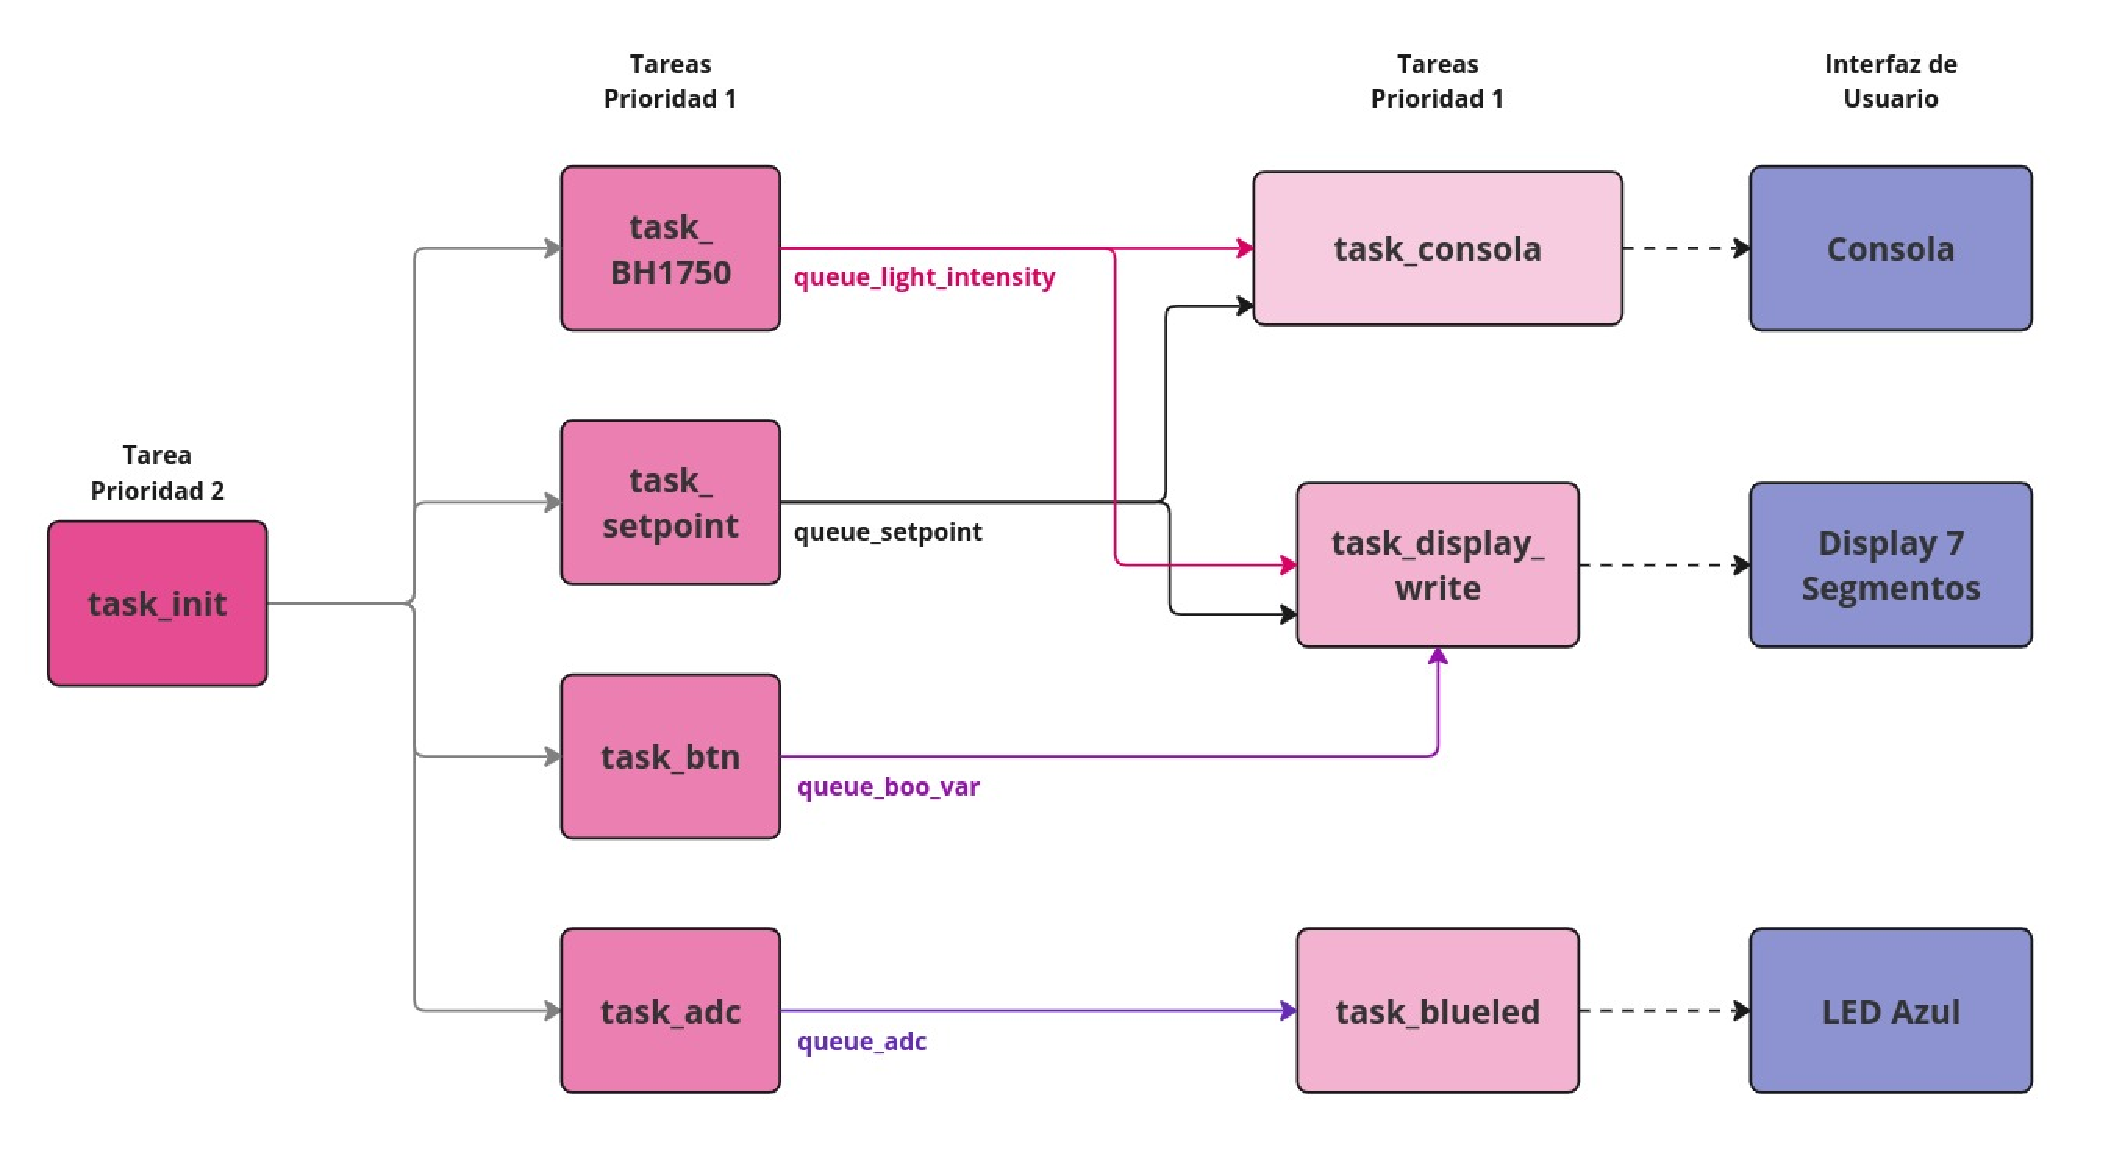
\includegraphics[width=\textheight, angle=90]{Diagrama de flujo_ProyectoIntegador.pdf}
        \label{fig:1}
    \end{figure}
\end{document}